\documentclass[../main.tex]{subfiles}
 
\begin{document}

To effectively evaluate the various algorithms, we conduct an experiment in which we test each approach on multiple instances of \prob. This section describes the code and the programming environment, the experimental process, and the results entailed. Additionally, this section discusses how the experiment compares to other experiments found in the literature. We utilize \cite{Barr1995}'s ``guidelines for testing and reporting'' throughout this section to adequately convey all relevant information to the reader.

\subsection{The Computing Environment}

The implementation code is fully detailed in Sections \ref{det:implementation}, \ref{sto:implementation}, and \ref{loc:implementation} and in Appendix \ref{app:code}, so we only briefly describe it here. We implemented two Python3 files: \texttt{main.py} and \texttt{data.py}. The former contains all algorithmic code; the latter contains only the problem instances used to evaluate the algorithms. Development occurred over a few weeks in April and May of 2019; we slightly revised the code in June 2019. 

Pseudocode for the algorithms employed is readily available online \cite{Hart1968, wikipedia:beam-search}; thus, we are confident the algorithms are correctly implemented. Previous experience in software development allows for easy, effective programming, and sufficient documentation means that we were able to revisit the code and ensure its correctness. The debugger in PyCharm, the \ac{ide} used to develop this code, allowed us to examine state variables during execution and validate the processes.

All code was written on a 2017 MacBook Pro running macOS Mojave 10.14.4. We used Python version 3.7.3 and PyCharm Professional version 2019.1 to write all of the implementation code. These resources allowed for portability and easy, on-the-go development of the code and of this report.

All tests were conducted within the PyCharm runtime environment. A simple \texttt{main} method iterates over the problem instances in \texttt{data.py}, and thus one execution of the program can evaluate all $10$ problem instances for one algorithm. The user can specific a different algorithm (from the choices \textit{deterministic}, \textit{stochastic}, and \textit{local}) within the \texttt{main} function.

All times were measured using Python3's \texttt{time} library. This library measures clock cycles of the computer and thus ensures timing accuracy across various systems.

Aside from selecting which algorithm one wishes to evaluate, the code is entirely hands-off. No tuning parameters must be set, and no input is required. Of course, the user can define new problem instances by appending to/modifying the data file.

\subsection{The Experimental Results}

This research intends to demonstrate whether or not the \ac{usaf} can feasibly solve \probs with a search algorithm. If so, the Air Force can guarantee survivability of its \acp{uav} while still conducting sufficient reconnaissance in an area with known sensor locations. If not, the Air Force must reevaluate the problem and perhaps consider other avenues for surveillance.

Of course, the search space for \probs is exceptionally large. We can see a tree representation of the search space in \figurename\ \ref{fig:search-tree}. A deterministic search, like A$^*$, which must often visit a huge number of the nodes in the tree to reach the globally-optimal solution, simply requires far too much computational time and resources to solve \probs for all but the smallest of problem instances. Stochastic and local search approaches do not require nearly the same amount of resources, but the sheer size of the search space ensures that neither approach is likely to reach the optimum. However, both the stochastic approach and the local one, if properly tuned, can reach a solution that meets some \textit{good enough} threshold, and both approaches can usually do so in a reasonable amount of time.

\begin{figure}
    \centerline{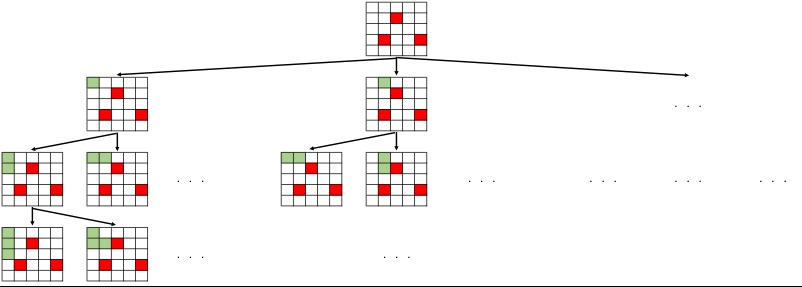
\includegraphics[width=\columnwidth]{search-tree.png}}
    \caption{A potential search tree for a \probs instance in which $n\geq 1$, $b\geq 3$, $|L|=3$, $r\approx 0.5$, and $d=5$. Clearly, the search tree quickly outgrows the available space in this report.}
    \label{fig:search-tree}
\end{figure}

\begin{figure}
    \centerline{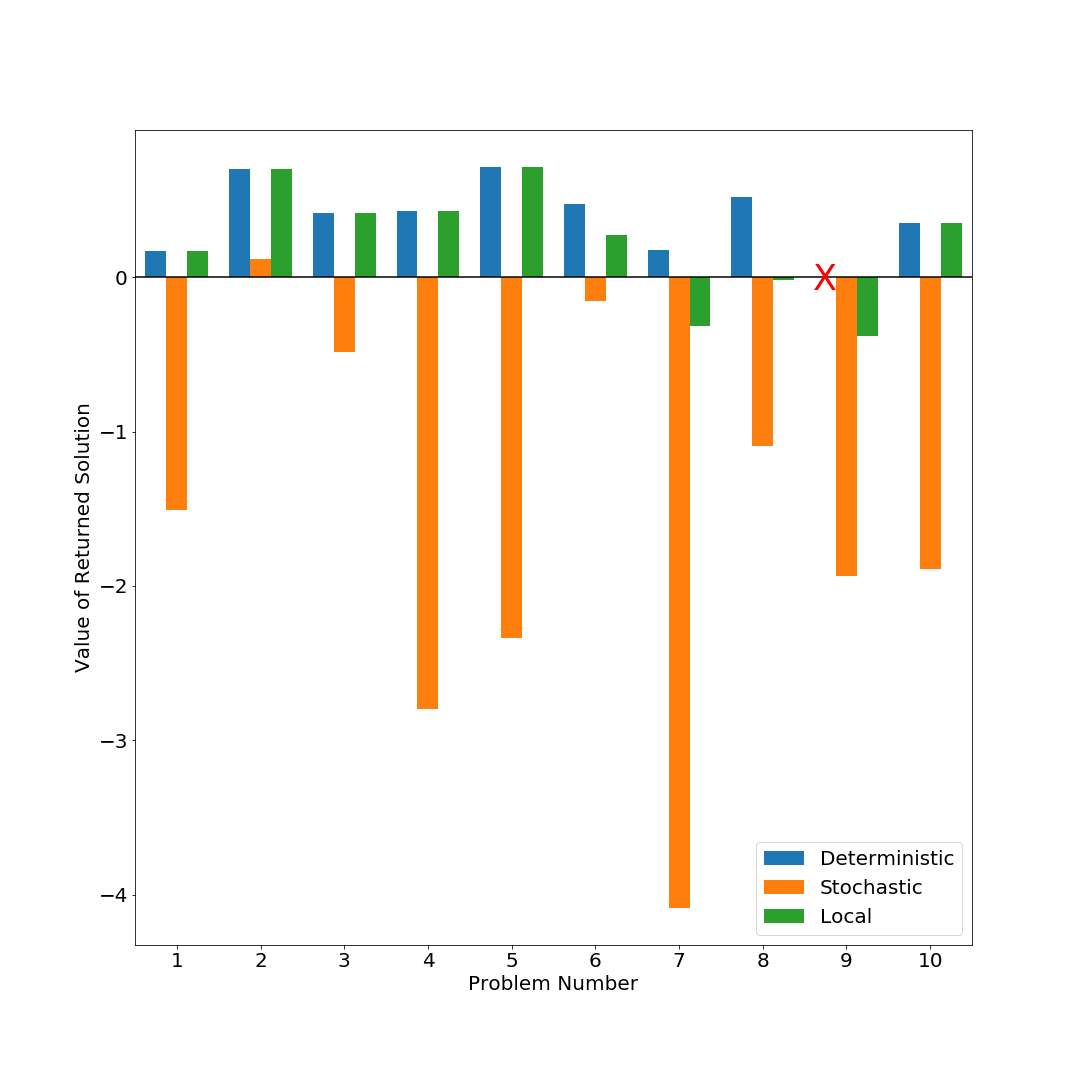
\includegraphics[width=\columnwidth]{bar-chart.png}}
    \caption{The results of the experiment. The deterministic algorithm's results are shown in blue; the stochastic algorithm's results are shown in orange; the local algorithm's results are shown in green. The deterministic algorithm did not solve Problem 9.}
    \label{fig:results-bar-chart}
\end{figure}

The results show this to be the case. We tested each algorithm on $10$ different (small) \probs instances. The exact parameters used for each problem instance can be seen in Table \ref{tab:det-results}. Tables \ref{tab:det-results}, \ref{tab:sto-results}, and \ref{tab:loc-results} show the execution time required for each of the $10$ problems for the deterministic, stochastic, and local approaches, respectively. The tables also display the value of the returned solution for every algorithm-problem instance combination. Clearly, the deterministic approach achieves the highest-valued solutions, but this requires significant execution time; problem 9 even failed to terminate (in $30$ minutes or less) for the deterministic approach! However, although the other two algorithmic techniques returned $10$ solutions each, most of those solutions are worse than the deterministic approach's solutions. As we can see in figure \ref{fig:results-bar-chart}, the stochastic algorithm performed much worse than the other two techniques. Sometimes, the local algorithm performed much like the deterministic approach, but it never performs much better, and it often performs much worse.

This illustrates a tradeoff between optimality and resources. This tradeoff is not unexpected, and thus we are not surprised that the fast algorithms perform worse than the slow one.

\begin{table*}
\caption{Implementation Results for the Deterministic Search Algorithm}
\centering
\label{tab:det-results}
\begin{tabular}{|l|l|l|l|l|l|l|l|}
\hline
\# & $n$ & $b$ & $L$                                             & $r$  & $d$ & Time ($s$)     & Value          \\
\hline
1  & 2   & 3   & (0.3, 1.8), (3.1, 2.7)                          & 1.2  & 4   & 0.064447       & 0.168319       \\
2  & 1   & 3   & (0.3, 1.8)                                      & 0.3  & 2   & 0.001389       & 0.700000       \\
3  & 1   & 4   & (1, 1)                                          & 3    & 2   & 0.001464       & 0.413514       \\
4  & 2   & 7   & (0.5, 0.9), (0.6, 1.1)                          & 1.1  & 3   & 0.026366       & 0.426602       \\
5  & 3   & 5   & (0.5, 1), (1.5, 1), (2.5, 1)                    & 0.5  & 3   & 0.063300       & 0.716667       \\
6  & 4   & 2   & (0.3, 1.8), (1.1, 2.9), (2.7, 2.7), (3.1, 2.7)  & 0.3  & 3   & 0.297092       & 0.474632       \\
7  & 2   & 7   & (-1, -1), (3.5, 2)                              & 3    & 4   & 0.147358       & 0.177236       \\
8  & 4   & 3   & (0.2, 0.1), (0.3, 0.7), (0.8, 3.4), (3.3, -0.2) & 0.6  & 4   & 7.490725       & 0.521721       \\
9  & 3   & 4   & (1, 1), (3, 1), (4, 1), (4.8, 5.1)              & 2.1  & 5   & $>$ 30 minutes & Did not finish \\
10 & 3   & 6   & (1.60, 0.75), (1.40, 3.65), (3.84, 2.70)        & 0.75 & 5   & 2.728232       & 0.350254       \\
\hline
\end{tabular}
\end{table*}

\begin{table*}
\caption{Implementation Results for the Stochastic Search Algorithm}
\centering
\label{tab:sto-results}
\begin{tabular}{|l|l|l|l|l|l|l|l|}
\hline
\# & Time ($s$) & Value     \\
\hline
1  & 0.015266   & -1.509787 \\
2  & 0.000855   & 0.120098  \\
3  & 0.001523   & -0.486486 \\
4  & 0.024772   & -2.799535 \\
5  & 0.041905   & -2.337500 \\
6  & 0.012181   & -0.152573 \\
7  & 0.051217   & -4.085834 \\
8  & 0.050550   & -1.095355 \\
9  & 0.110520   & -1.936070 \\
10 & 0.075914   & -1.892918 \\
\hline
\end{tabular}
\end{table*}

\begin{table*}
\caption{Implementation Results for the Local Search Algorithm}
\centering
\label{tab:loc-results}
\begin{tabular}{|l|l|l|l|l|l|l|l|}
\hline
\# & Time ($s$) & Value \\
\hline
1  & 0.009594 & 0.168318  \\
2  & 0.000691 & 0.700000  \\
3  & 0.000796 & 0.413513  \\
4  & 0.012163 & 0.426602  \\
5  & 0.011291 & 0.716666  \\
6  & 0.017952 & 0.271139  \\
7  & 0.026866 & -0.313384 \\
8  & 0.060396 & -0.018886 \\
9  & 0.112361 & -0.382878 \\
10 & 0.149047 & 0.350254  \\
\hline
\end{tabular}
\end{table*}

\subsection{Results Analysis}

Results indicate that the algorithms implemented in this research fall into one of two classes:

\begin{enumerate}
    \item Those that identify strong results but, due to the size of the search space, are unable to terminate for large problem instances; and
    \item Those that terminate in a reasonable time but with (usually) poor solutions.
\end{enumerate}

\noindent It seems that neither A$^*$ nor \ac{lbs} nor \ac{sbs} are suitable techniques for solving \prob, at least where the \ac{usaf} is concerned. For this reason, the military should consider other multi-domain optimization techniques, including some of those discussed in Appendix \ref{app:other-search}. It's likely that many more approaches -- including those that vastly outperform the techniques employed here -- are hidden in the literature. Additionally, the \ac{usaf} best knows its problem domain, so it's likely that those responsible for solving \probs can better tune the heuristic functions.

\end{document}